\chapter{Resultados}
\label{resultadosiniciais}


Este capítulo apresenta os resultados iniciais de dois experimentos distintos, cada um focado em explorar aspectos importantes para este trabalho. Inicialmente, abordaremos o desenvolvimento de um compilador, seguido por uma investigação prática sobre técnicas de \textit{ray tracing}.


O experimento com o compilador visa proporcionar uma compreensão mais profunda  do desenvolvimento de compiladores. Isso foi realizado através da escolha de uma linguagem simples para implementação, que será chamada \texttt{SimpleLang}. Por ser uma linguagem com menos regras de sintaxe que o \LaTeX, é possível a exploração do processo de compilação incluindo a tokenização, criação da árvore sintática e interpretação do código-fonte por meio dessa árvore sintática. Esse compilador foi desenvolvido sem o uso de bibliotecas externas, o que amplia o entendimento sobre os fundamentos do desenvolvimento de compiladores.




Por outro lado, o experimento com o \textit{ray tracing} representa um estudo prático sobre BRDFs e a linguagem Odin. Embora o objetivo principal seja compreender melhor o funcionamento das funções de distribuição de reflectância bidirecional (BRDFs), há uma conexão futura com o compilador, pois há a possibilidade de integração do \textit{ray tracer} implementado como um pré-visualizador das BRDFs. No entanto, o foco principal permanece no compilador, enquanto o \textit{ray tracer} serve como uma oportunidade para explorar as capacidades da linguagem Odin e aplicar os conceitos de radiometria.


Esses experimentos se complementam, proporcionando uma abordagem que explora tanto os aspectos teóricos quanto práticos relacionados ao desenvolvimento de compiladores e à aplicação de conceitos como BRDFs


\section{Parser e Lexer em Odin} \label{parser}


Desenvolvemos um \textit{lexer}, \textit{parser} e interpretador para uma linguagem simples chamada \texttt{SimpleLang}, juntamente com sua gramática, utilizando o Pratt \textit{Parsing} na linguagem de programação Odin. O repositório pode ser encontrado em \url{https://github.com/evertonse/pratt-parser}. Esse \textit{parser} é implementado por descida recursiva, o que significa que cada regra de produção tem uma função de análise associada. A implementação prioriza a simplicidade de código e a clareza de ideias, com extensos comentários para auxiliar na compreensão. Isso é importante, pois esse \textit{parser} será modificado para aceitar \textit{tokens} e sintaxe de \LaTeX.


\subsection{Parser}


Ao contrário dos \textit{parser} de descida recursiva tradicionais, que muitas vezes exigem várias chamadas de função aninhadas para cada nível de precedência, o nosso \textit{parser} organiza as funções de análise hierarquicamente com base na precedência do operador, como demonstrado no \autoref{alg-pratt-parsing}. Esse código é a parte principal do \textit{parsing} de expressões. Nessa implementação usamos a notação original de Pratt \cite{pratt}, as funções \texttt{null\_denotations} e \texttt{left\_denotations} são equivalentes as funções \texttt{token.prefixo} e \texttt{token.infixo} declaradas no \autoref{alg1}, respectivamente. Os pacotes desse projeto estão definidos na \autoref{folder}.




\begin{codigo}[H]
  \caption{\small Parsing de expressão em código Odin.}
        \label{alg-pratt-parsing}
  \begin{lstlisting}[language=C]


parse_expr :: proc(prec_prev: i64) -> ^Expr {
    /* expressions that takes nothing (null) as left operand */
    left := parse_null_denotations() 
    /*
    . if current token is left associative or current token has higher precedence
    . than previous precedence then stay in the loop, effectively creating a left leaning
    . sub-tree, else, we recurse to create a right leaning sub-tree.
    */
    for precedence(peek()) > prec_prev + associativity(peek())  {
        /* expressions that needs a left operand such as postfix, mixfix, and infix operator */
        left = parse_left_denotations(left)
    }
    return left
}


  \end{lstlisting}
\end{codigo}


\begin{figure}[H]
        \caption{\label{folder} \small Estrutura de pacotes do compilador.}
        \begin{center}
            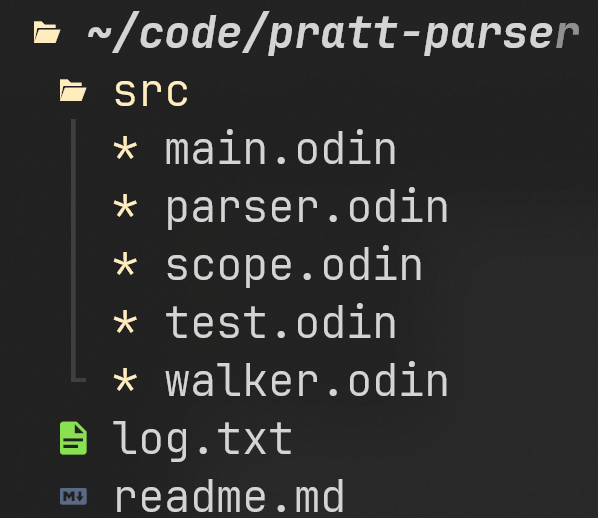
\includegraphics[scale=0.5]{./Imagens/folder_structuer_odin_parser_lexer.png}
        \end{center}
\end{figure}


\subsection{Gramática}

Para formalizar a gramática da linguagem de entrada (\texttt{SimpleLang}) deste compilador, definimos suas regras no \autoref{lst-gramatica}. Um exemplo de código-fonte válido em \texttt{SimpleLang} é apresentado no \autoref{code-gramatica}.


\begin{codigo}[htb]
        \caption{\small Exemplo código escrito na linguagem \texttt{SimpleLang}. }
        \label{code-gramatica}
  \begin{lstlisting}[language = python]
    epsilon = 0.001; # proximidade em float


    abs = fn(a) a lt 0 or a lt -0 ? -a : a;


    float_close = fn(a, b) 
        abs(a - b) lt epsilon ? 
            1 : 0;


    # Classical fibonacci
    fib = fn(n)  
        float_close(n, 0) ? 
            0
        :float_close(n, 1) ?
            1
        :fib(n-1)  + fib(n-2);


    fib(10)  # Ultima expressao significa retorno do main
  \end{lstlisting}
\end{codigo}

\begin{codigo}[H]
        \caption{\small Gramática para \texttt{SimpleLang}.}
        \label{lst-gramatica}
% \begin{lstlisting}[numbers=none, frame=none,caption=,label=]
\begin{lstlisting}[numbers=none, frame=none]
start = assign* expr ;


expr = prefix expr 
       | expr postfix  
       | expr infix expr 
       | expr '?' expr ':' expr
       | call
       | NUMBER
       | IDENTIFIER
       ;


assign = IDENTIFIER '=' expr ';'
         | IDENTIFIER '=' 'fn' (' params ')' expr ';'
         ; 


call = expr '(' args ')';
args = expr
        | expr ',' args
        | 
        ;
params = IDENTIFIER
         | IDENTIFIER ',' params
         | 
        ;


postfix = '+' | '-' | '~' | '!';
prefix  = '+' | '-' | '~' | '!';
infix   = '+' | '-' | '*' | '/' | '^'
            | 'eq' | 'lt' | 'gt' | 'or' | 'and'
            ;
\end{lstlisting}
\end{codigo}


  Na definição da gramática (\autoref{lst-gramatica}), utilizamos uma notação leve de sintaxe para representá-la. Palavras com todas as letras minúsculas são não-terminais, enquanto palavras entre aspas simples representam literalmente um \textit{token} com esse conteúdo. Palavras em letras maiúsculas representam um \textit{token} que pode variar, mas mantém o mesmo significado semântico. Por exemplo, NUMBER pode ser 2.0 ou 1.0, mas nas regras de produção eles são tratados de maneira idêntica. O símbolo ``$*$'' indica zero ou mais ocorrências, ``$()$'' indica agrupamento para aplicar um operador a ele, ``$|$'' simboliza o início de uma regra alternativa para o mesmo não-terminal e ``$=$'' indica uma produção.

% \begin{lstlisting}[frame=bt,numbers=none]




Essa gramática define regras para expressões, atribuições, chamadas de função e vários operadores, como \texttt{postfix}, \texttt{prefix} e \texttt{infix}, com o intuito de criar uma vasta coleção de operadores com diferentes precedências para facilitar a transição da sintaxe de \texttt{SimpleLang} para a sintaxe \LaTeX\  futuramente.






\subsection{Tabela de Símbolos}


Nesse projeto, foi desenvolvido também uma tabela de símbolos simples, cuja implementação será reaproveitada na análise semântica e na geração de código GLSL futuramente. A implementação da tabela de símbolos fornecida aqui é baseada em uma estrutura de escopo hierárquico, onde cada escopo mantém um mapeamento entre os nomes dos símbolos e seus atributos correspondentes. No \autoref{struct-symbol} temos a estrutura \texttt{Scope}, que representa um mapeamento de nomes para objetos de símbolo dentro de um \textbf{único escopo}, e também a estrutura \texttt{Scope\_Table}, que mantém uma \textbf{pilha de escopos}, permitindo aninhamento.


\subsubsection{Estrutura de Símbolos}


Cada objeto na tabela de símbolos é representado pela estrutura \texttt{Symbol}, que contém os seguintes atributos:
\begin{itemize}
    \item \texttt{name}: o nome do símbolo.
    \item \texttt{val}: o valor associado ao símbolo (para variáveis).
    \item \texttt{is\_function}: um sinalizador booleano indicando se o símbolo é uma função.
    \item \texttt{params}: uma lista de \textit{tokens} representando os parâmetros da função.
    \item \texttt{body}: um ponteiro para a expressão que representa o corpo da função (se aplicável).
\end{itemize}




\begin{codigo}[htb]
\caption{\small Código da estrutura de símbolos escrito em Odin.}
\label{struct-symbol}
\begin{lstlisting}[language=C]
Scope :: #type map[string]Symbol
Scope_Table :: [dynamic]Scope


Symbol :: struct  {
    name : string,
    val: f64,
    is_function: bool,
    params: []Token,
    body: ^Expr,
}

\end{lstlisting}
\end{codigo}


\subsubsection{Gerenciamento de Escopo}

A tabela de símbolos fornece funções para gerenciar escopos, incluindo:
\begin{itemize}
    \item \texttt{scope\_enter}: entrar em um novo escopo, anexando-o à pilha de escopos.
    \item \texttt{scope\_exit}: sai do escopo atual, removendo-o da pilha de escopos e o retornando.
    \item \texttt{scope\_reset}: redefine a tabela de símbolos limpando todos os escopos.
    \item \texttt{scope\_get}: recupera um símbolo da tabela de símbolos pelo seu identificador.
    \item \texttt{scope\_add}: adiciona um novo símbolo ao escopo atual.
\end{itemize}




Essa tabela de símbolos será adaptada para a fase de geração de código e tradução adequada do código-fonte em \textit{shaders} GLSL.




\subsubsection{Estrutura da Árvore de Sintaxe}
Nesta seção, apresentamos os tipos de nós que compõem a árvore de sintaxe abstrata (AST), utilizada no compilador da linguagem \texttt{SimpleLang}. A estrutura da AST é definida com vários tipos de nós para capturar diferentes elementos da sintaxe. Diferente da gramática definida no \autoref{lst-gramatica}, aqui os nós são representados em nível de código. A seguir, listamos a representação semântica de cada nó:


\begin{itemize}
\item \textbf{Ast}: a estrutura base para todos os nós da AST.
\item \textbf{Start}: representa o ponto de partida do programa, contendo uma sequência de atribuições seguidas de uma expressão.
\item \textbf{Assign}: representa atribuições de variáveis, incluindo um identificador, operador de atribuição e expressão.
\item \textbf{Assign\_Function}: estende \textit{Assign} e representa definições de funções, incluindo parâmetros.
\item \textbf{Expr}: representa expressões de maneira abstrata, servindo como a estrutura base tipos concretos de expressões.
\item \textbf{Expr\_Identifier}: representa identificadores dentro de expressões.
\item \textbf{Expr\_Number}: representa literais numéricos dentro de expressões.
\item \textbf{Expr\_Grouped}: representa expressões agrupadas dentro de parênteses.
\item \textbf{Expr\_Prefix}: representa operações unárias (prefixo).
\item \textbf{Expr\_Infix}: representa operações binárias (infixo).
\item \textbf{Expr\_Postfix}: representa operações unárias (sufixo).
\item \textbf{Expr\_Mixfix}: representa operações ternárias.
\item \textbf{Expr\_Function\_Call}: representa chamadas de função com argumentos.


\end{itemize}


\subsection{Implementação do Padrão de Visitante}


O padrão visitante foi empregado para percorrer e operar em uma AST. Três procedimentos implementam esse padrão e manipulam a AST:


\begin{itemize}
  \item \textbf{walker\_interp}: interpreta a AST, calculando o valor numérico das expressões.
  \item \textbf{walker\_paren}: gera uma representação de \textit{string} entre parênteses da AST, auxiliando na legibilidade e garantindo a ordem correta de avaliação.
  \item \textbf{walker\_print}: imprime os nós da AST e seus atributos, facilitando a depuração e compreensão da estrutura da AST.
\end{itemize}


\subsection{Testes}


Foi desenvolvida uma série de testes que  abrangem vários aspectos da funcionalidade do \textit{parser}, incluindo geração de árvore de sintaxe, precedência de operadores e interpretação semântica.


\subsubsection{Geração de Árvore de Sintaxe}


Um aspecto crucial dos testes envolve verificar a correta geração de árvores sintáticas a partir de expressões de entrada. Os testes são projetados para cobrir diferentes cenários, incluindo operações aritméticas simples, expressões complexas com sub-expressões aninhadas e chamadas de funções. São eles:


\begin{itemize}
    \item O manuseio correto de operadores unários e binários, garantindo a precedência e associatividade adequadas.
    \item A representação precisa de chamadas de função e seus argumentos dentro da árvore de sintaxe.
    \item O agrupamento adequado de expressões dentro de parênteses para confirmar regras de precedência.
\end{itemize}

\subsubsection{Interpretação Semântica}

Além da geração da árvore de sintaxe e da definição de precedência de operadores, foram realizados testes para garantir a interpretação semântica das expressões. Isso envolve avaliar as entradas e comparar a saída com os valores esperados. Quanto à verificação de tipos, é simples: cada variável pode ser uma função ou um número. Portanto, permitimos apenas operadores entre números e, além disso, booleanos também são considerados números, sendo $0$ interpretado como falso e $1$ como verdadeiro. Os testes de interpretação semântica realizados para \texttt{SimpleLang} abrangem:


\begin{itemize}
    \item Avaliar expressões aritméticas envolvendo constantes, variáveis e chamadas de função recursivas.
    \item Verificar o comportamento de expressões condicionais (por exemplo, operador ternário) sob diferentes condições.
\end{itemize}


Ao testar geração de árvore de sintaxe, precedência de operadores e interpretação semântica, a implementação do Pratt \textit{Parsing} foi validada quanto à correção e confiabilidade, pois obteve um desempenho robusto em vários cenários de entrada.

